%%%%% Document Setup %%%%%%%%

\documentclass[12pt, twocolumn]{revtex4}    % Font size (12pt) and column number (one or two).

\usepackage[a4paper, left=2.5cm, right=2.5cm, top=2.5cm, bottom=2.5cm]{geometry}  % Defines paper size and margin length

\usepackage{ragged2e}

\renewcommand{\baselinestretch}{1}     % Defines the line spacing

\usepackage{subcaption}
\usepackage[font=small, labelfont=bf, justification=justified, format=plain, singlelinecheck=off]{caption}\captionsetup{compatibility=false, justification=justified,}

\usepackage{graphics,graphicx,epsfig,ulem}	% Makes sure all graphics works
\usepackage{amsmath} 						% Adds mathematical features for equations

\usepackage{etoolbox}                       % Customise date to preferred format
\makeatletter
\patchcmd{\frontmatter@RRAP@format}{(}{}{}{}
\patchcmd{\frontmatter@RRAP@format}{)}{}{}{}
\renewcommand\Dated@name{}
\makeatother

\usepackage{fancyhdr}
 
\usepackage[UKenglish]{babel}% http://ctan.org/pkg/babel

\pagestyle{fancy}                           % Insert header
\renewcommand{\headrulewidth}{0pt}
\lhead{\small Jacky Cao}                        
\rhead{\small The relation between stars and gas in distant galaxies}                

\def\thesection{\arabic{section}}
\def\thesubsection{\alph{subsection}}

\def\bibsection{\section*{References}}        % Position reference section correctly

\usepackage{tabularx}

%%%%% Document %%%%%
\begin{document}                     


\title{The relation between stars and gas in distant galaxies} 
\date{Submitted: \today{}}
\author{Jacky Cao}
\affiliation{\normalfont Level 4 Project, MPhys Physics\\ Supervisor: Dr.~Mark Swinbank\\ Department of Physics, Durham University}

\begin{abstract}              
 
 Observing any galaxy in the universe will yield the fact that it contains stars and also gas. The dynamics of both can be explored by observing galaxies and collecting spectroscopic data. 
 
Abstract abstract abstract abstract abstract abstract abstract abstract abstract abstract abstract abstract abstract abstract abstract abstract abstract abstract abstract abstract abstract abstract abstract abstract abstract abstract abstract abstract abstract abstract abstract abstract abstract abstract abstract abstract abstract abstract abstract abstract abstract abstract abstract abstract abstract abstract abstract abstract abstract abstract abstract abstract abstract abstract abstract abstract abstract abstract abstract abstract abstract abstract abstract abstract abstract abstract abstract abstract abstract abstract abstract abstract abstract abstract abstract abstract abstract abstract abstract abstract abstract abstract 

\end{abstract}

\maketitle
%\thispagestyle{plain} % produces page number for front page

\tableofcontents
%\let\toc@pre\relax
%\let\toc@post\relax

\newpage

\section{Introduction} 

Amongst the different types of cosmic structure within our universe, galaxies can be described as the most unique and diverse. With each containing countless numbers of stars and vast amounts of gas, dust, and dark matter \cite{carroll_astro}, it would certainly be surprising if these various objects were found to not be connected in any way.

Through observational astronomy the internal structure of galaxies and the motions of their inner objects can be studied and understood. With approximately ($2.0^{+0.7}_{-0.6}$) $\times 10^{12}$ galaxies in the universe up to $z=8$ which in principle could be observed \cite{conselice_galaxynumber}, there is definitely not a lack of choice. What is important is how these objects are observed and how the collected data is later analysed. 

% Through observations of these galaxies, their structure and the motions of the objects within them can be studied to a great depth. As an example, if we took optical measurements of the stellar population, we could use that information to infer and estimate the potential age of the galaxy. We know that redder stars are older and bluer stars represent a younger set of objects \cite{carroll_astro}. Or if we wanted to know about the material composition or even the distance to a certain galaxy, we could split the collected light in a spectrograph to produce a spectrum. Values of redshift and the content of a galaxy can then be obtained by looking at the absorption and emission lines \cite{carroll_astro}.

It is additionally significant to understand what a galaxy generally is and how they can be defined and placed into different categories. Once an appreciation is built for the galactic classification, the intricacies of motions and inter-relationships can be explored further. 

%  for example how a galaxy evolves from the early stages of being a gas cloud to the eventual relation of the stellar population to that gas.

\subsection{Galactic classification}

As stated previously, a galaxy can be quite broadly defined as a collection of gas, dust, stars and dark matter. But if a large enough sample was observed then one would begin to see that they can be grouped and classified together.

The most general categorisation is called the \textit{Hubble Sequence} or the \textit{Hubble Tuning Fork} \cite{carroll_astro}. Developed by Edwin Hubble in 1926, galaxies can be roughly divided into ellipticals, spirals and irregulars (Fig. \ref{fig:hubble_tuning_fork}). With early Hubble type ellipticals along the horizontal handle, then the two prongs contain normal and barred spirals (later Hubble types), and irregulars as the third category. What can be seen from the Tuning Fork is a summarised view of the main galaxy types, however in reality there are more than the 11 named.

\begin{center}
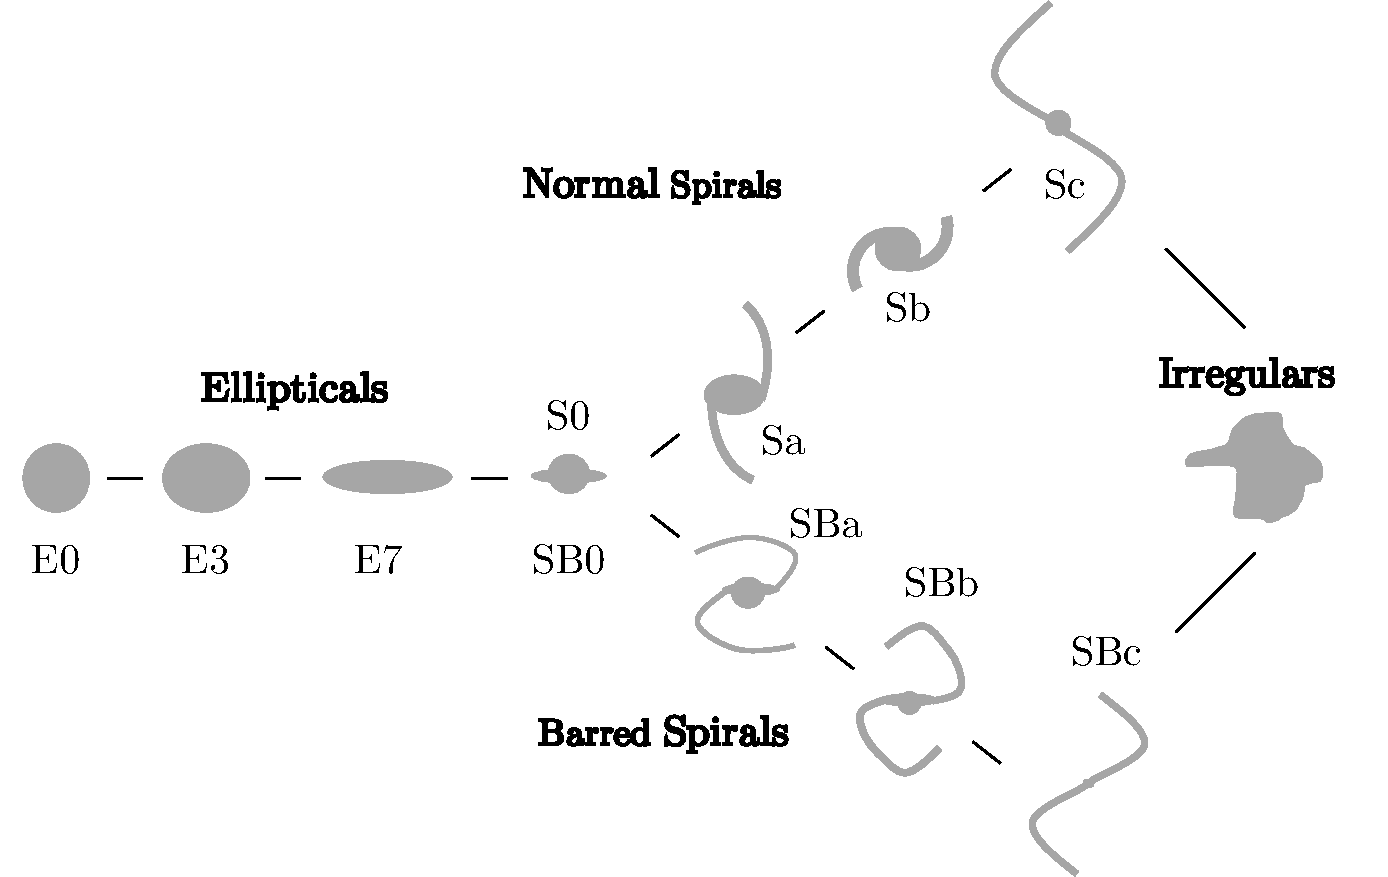
\includegraphics[width=1.0\linewidth]{introduction/hubble_tuning_fork}
\captionof{figure}[Hubble Tuning Fork]{The Hubble Sequence displays the different morphologies of galaxies, they can be classified into three general groups: ellipticals, spirals, and irregulars. The former two can be broken up further, and from the diagram one can see an example pictogram and the respective classification name. \\ (\textit{This diagram has been adapted from An Introduction to Modern Astrophysics} \cite{carroll_astro}.)}
\label{fig:hubble_tuning_fork}
\end{center}

The sequence itself does not show the evolution of the galaxies, rather it provides a way to view the different potential morphologies. So then, what does each grouping from the sequence actually represent? 

Starting with the most broad, irregulars are objects which do not fall into the two main galaxy types (ellipticals and spirals). In fact they themselves can be split into two sub-categories depending on if a particular galaxy could be seen to have structure, such as spiral arms \cite{carroll_astro}. If they did then they would be Irr I galaxies, and if they appeared to be extremely disorganised then Irr II. Generally, irregulars are not particularly large, their diameters typically range from 1 to 10 kpc, and they have an absolute B-band magnitude of $-13$ to $-20$ mag.

% Some astronomers even argue that there is not a strong particular need for this grouping as these galaxies can fall into the spherical type \cite{carroll_astro}.

This classification by appearance can easily be extended to ellipticals and spirals, and their individual component composition can be studied and explored as well. 

With ellipticals, they span from being virtually spherical (E0) to highly flattened (E7) collections of objects and material \cite{moore_databook}. Through observations of their stars, it can be seen that the majority of them are old and red types. This may be attributed to the amount of gas used in the initial stages of galactic stellar formation. If a larger proportion was used up initially then current observations would should the stellar-birthrate in ellipticals to be low \cite{carroll_astro}. This could additionally explain the lack of disks which can otherwise be seen in spiral galaxies, if there is not enough surrounding material then the disk and arms features would not be able to form.

Exploring spirals, they can be described as being composed of a central nucleus with a surrounding disk of material. This disk contains denser regions which forces material to collapse and coalesce to form additional features. One of the characteristics leads to a supplemental classification, and that is whether the nucleus has a ``bar'' running through it. Observing and comparing the two different types, one finds that barred spirals appear to be more elongated along the bar axis than their non-barred counterparts. 

The other main attribute for spiral galaxies are the protruding arms surrounding the main bulge \cite{carroll_astro}. In the later type spirals (Sc and SBc) they have arms which are more loosely wound than the earlier types (Sa and SBa) \cite{moore_databook}. It can be seen implied that with more available ``raw'' gas and dust \cite{carroll_astro}, spirals in their various forms could be assumed to have an overall younger stellar population.

It is within the arms of spiral galaxies that new stars are found to be created, however stellar birth is definitely not limited to just these regions. Inside the spiral structure the gravitational field allows for angular momentum to be transported outwards. Older and less massive stars in the galaxy produce a gravitational field which eventually leads to the shocking of interstellar gas \cite{binney_galaxies}. As a result the density of the gas in the arms increase and certain regions then collapse to form new, young, blue, and massive stars. 

There is therefore a range in the stellar population age of spiral galaxies. The spiral arms contain young stars whilst the central nucleus is akin to that of elliptical galaxies, where they have an older population of stars and fewer new stars are being created \cite{carroll_astro, binney_galaxies}.

These then are the general characteristics of galaxies, and whilst they can be classified based on their appearance, it is through studying their stellar populations that our understanding of them will improve. 

% TODO if I am going to discuss galactic formation, should I have mentioned the earlier detail on how ellipticals form stars early on in the galaxies' history? 

\subsection{Galactic stellar formation}

% this section shouldn't be called galactic stellar formation

One could argue that the main backbone in any galaxy lies with the gas and dust, as without them there would be no stars and galaxies would simply not exist. There are many models which aim to provide an explanation for galactic evolution, from an initial proto-nebulae to potential structure. It would be difficult to explain them all, but it would be beneficial to address some issues which would have to be answered by a comprehensive theory. 

One such problem is deciding if an initial nebula collapses in free-fall or whether it goes through a slow and dissipative collapse \cite{carroll_astro}. If the time taken to cool the nebula significantly (cooling timescale) is much less than the time taken for free-fall, then the cloud would not be pressure supported and the collapse would be a rapid free-fall. On the other hand, if the cooling time exceeds the free-fall time then a rapid collapse cannot occur as the gas cannot radiate its energy away fast enough, so the gravitational potential energy released from collapse will heat the nebula adiabatically. 

This is important to understand as from the heated and collapsed gas, the first stars can then be produced. It is not surprising then that a theory for galactic evolution should also be able to explain the rate of star formation. This rate can be described as a stellar birthrate function, $B(M,t)$, and be expressed as,
\begin{equation}
B(M,t)dM dt = \psi (t) \xi (M) dM dt, 
\label{eqn:stellar_birth_rate}
\end{equation}

where $\psi(t)$ is the star formation rate (SFR), $\xi (M)$ is the initial mass function (IMF), $M$ is the stellar mass, and $t$ is the time \cite{carroll_astro}. 

Describing what each term physically represents, $B(M,t)$ is the number of stars per unit volume with masses between $M$ and $M+dM$ which are formed out of the interstellar medium (ISM) between time $t$ and $t+dt$, $\psi(t)$ is the rate per unit volume at which mass in the ISM is converted into stars, and $\xi(M)$ is the relative number of stars which form in each mass interval \cite{carroll_astro}. 

Various problems arise when several researchers provide different assumptions for the different terms in the equation \cite{carroll_astro}. Some say that the SFR is time-independent, whilst others describe it as exponentially decreasing with time, and a few even argue that the SFR is proportional to a power of the surface mass density of the galactic disk. Then take the IMF, there is disagreement on the exact form it takes, some model it to be a power-law as a function of mass, but it is not clear if it also varies with time or location.

Through contentious debate and research, astronomers can continue to build these different models and theories which attempt to explain galactic evolution. Whilst on the other hand, the evolution of the stars themselves are known and understood to a greater degree. 

In a brief overview: stars are born from an interstellar medium where the gas and dust coalesce, collapse and heat-up until a protostar is created. Depending on the initial mass of material used, the star can then take various paths which will affect its subsequent future \cite{mccoy_space_sciences}. To view the different stages of stellar evolution, Hayashi tracks and the Hertzsprung-Russell diagram can be paired together \cite{carroll_astro}. In doing so, one would find that the majority of stars lie on the main-sequence, including our own Sun. 

The classification of stars can be made with the \textit{Harvard Spectral Classification} where stars are classed by their spectral types (Table \ref{table:spectral_classification}). It essentially orders stars by their observed temperature and their internal composition. If a star's spectra was observed, it could be identified by the absorption and emission features found in the sequence.    
\begin{center}
\begin{tabular}{c@{\hskip 20pt}c} 
 \hline
 \textbf{Type} & \textbf{Colour and notable lines} \\ [0.5ex] 
 O & Hot blue-white (He II, He I) \\
 B & Hot blue-white (He I, H I ) \\
 A & White (Balmer, Ca II) \\
 F & Yellow-white (Ca II, Fe I, Cr, I) \\
 G & Yellow (Ca II, Fe I,  \\
  & neutral metals) \\
 K & Cool orange (Ca II H and \\ 
  & K, metals) \\
 M & Cool red (TiO, VO, neutral \\
  & metals) \\
 L & Very cool, dark red, infrared \\
  & (Molecular absorption, CrH, \\
  & FeH, H$_2$O, CO, Na, K, Rb, Cs) \\
 T & Coolest, infrared (CH$_4$, CO) \\
 \hline
\end{tabular}
\captionof{table}[Harvard Spectral Classification]{The Harvard Spectral Classification for stellar objects. Stars can be defined by their colour and from the features seen from their spectra. Provided in the table are the spectral type, the associated colour plus the main emission or absorption lines to consider. \\
(\textit{This table is adapted from a version from An Introduction to Modern Astrophysics} \cite{carroll_astro}.)}
\label{table:spectral_classification}
\end{center}

% If I need more discussion space, I could place the table in an appendix?

This is therefore one of ways to study the stellar population of a galaxy as the signatures of different spectral types can be matched up in the spectra of a particular galaxy. 

It is clear then that observational data would be required for own study of galaxies and the internal motions of the objects within them. 

\subsection{Galactic data} 

For an investigation of galaxies, one would have to collect data optically and also spectroscopically. The former would be useful as it would allow for a quick identification of the galaxy based on its appearance, this could then be used to infer whether a galaxy would be worth studying. Spectroscopic data on the other hand would be important to collect as a variety of information could be obtained such as the type of stars within a galaxy, the types of gas in surrounding clouds, and also the redshift. 

Astronomers on a daily basis employ an assortment of telescopes and spectrographs, but there are just a few particular instruments which are worth discussing as they have produced remarkable datasets and results.

\subsubsection{HUDF}

The Hubble Space Telescope (HST) has been operating since April 1990 and for the duration of that time it has collected over 50 terabytes of data \cite{mccoy_space_sciences}. From observing nebulae to attempts to detect extra-solar planets, HST has been used in a variety of searches. However, one of the most impressive and insightful uses of HST was the collection of the long-exposures taken in 1996 to produce the Hubble Deep Field (HDF). 

Through a combination of its visible and infrared cameras, the HDF was produced by piecing together different datasets which were collected over a period of 10 consecutive days \cite{mccoy_space_sciences, williams_hdp}. The four-band, 0.5 million s exposure revealed sources with redshifts $z>1$ which would have been difficult to view from ground-based observations \cite{beckwith_hudf}. 

% Expand on this section in the actual report i.e. the implications of HDF
% What regions of space was used to create the HDF? 

It is therefore unsurprising that another attempt was made in 2011 which resulted in the Hubble Ultra Deep Field (HUDF). This survey utilised 1 million s of exposure time on an 11 arcmin$^2$ area in the southern sky. Viewed again with four different filters, this survey resulted in at least 10,000 objects being detected in the field \cite{beckwith_hudf}. With a large majority being galaxies, the HUDF would be a prime dataset for a study of them as one would have a large range of candidates spanning a large proportion of the universe's history. 

% Should probably talk more about the HUDF and what the specs of it actually are, I'm just currently a bit conscious on the amount of space which I have left 

% why was the HUDF deep field commisioned?

\subsubsection{MUSE}

In addition to optical observations, to truly study the HUDF objects, spectroscopic data must also be employed. One particular instrument which was used to acquire data on the HUDF region is the Multi-Unit Spectroscopic Explorer (MUSE) mounted to the Nasmyth platform on the Very Large Telescope (VLT) \cite{bacon_muse_proposal}. 

% provide some more history and specs for MUSE, reasons as to why it was commissioned 

The MUSE Hubble Ultra Deep Field Survey was performed over a two year timeframe from September 2014 to February 2017 \cite{bacon_muse_hudf}. It made use of 137 h of observation time and covers 90\% of the HUDF region. A composite mosaic of nine fields, the final 3D data cube represents the deepest spectroscopic survey ever performed. Both HST and MUSE HUDFs can be optically compared together, the latter is achieved by collapsing the cube axis containing the spectroscopic data into three components representing (R,G,B). It can be seen (Figure \ref{fig:hst_muse_hdf}) 

% TODO what is MUSE, where it is on the VLT, problems, limitations of MUSE - why it is useful...etc

% what are the three dimensions of the 3D data MUSE cube? then what are the units of each dimension??

\onecolumngrid

\begin{figure}
  \begin{subfigure}[b]{0.4\textwidth}
    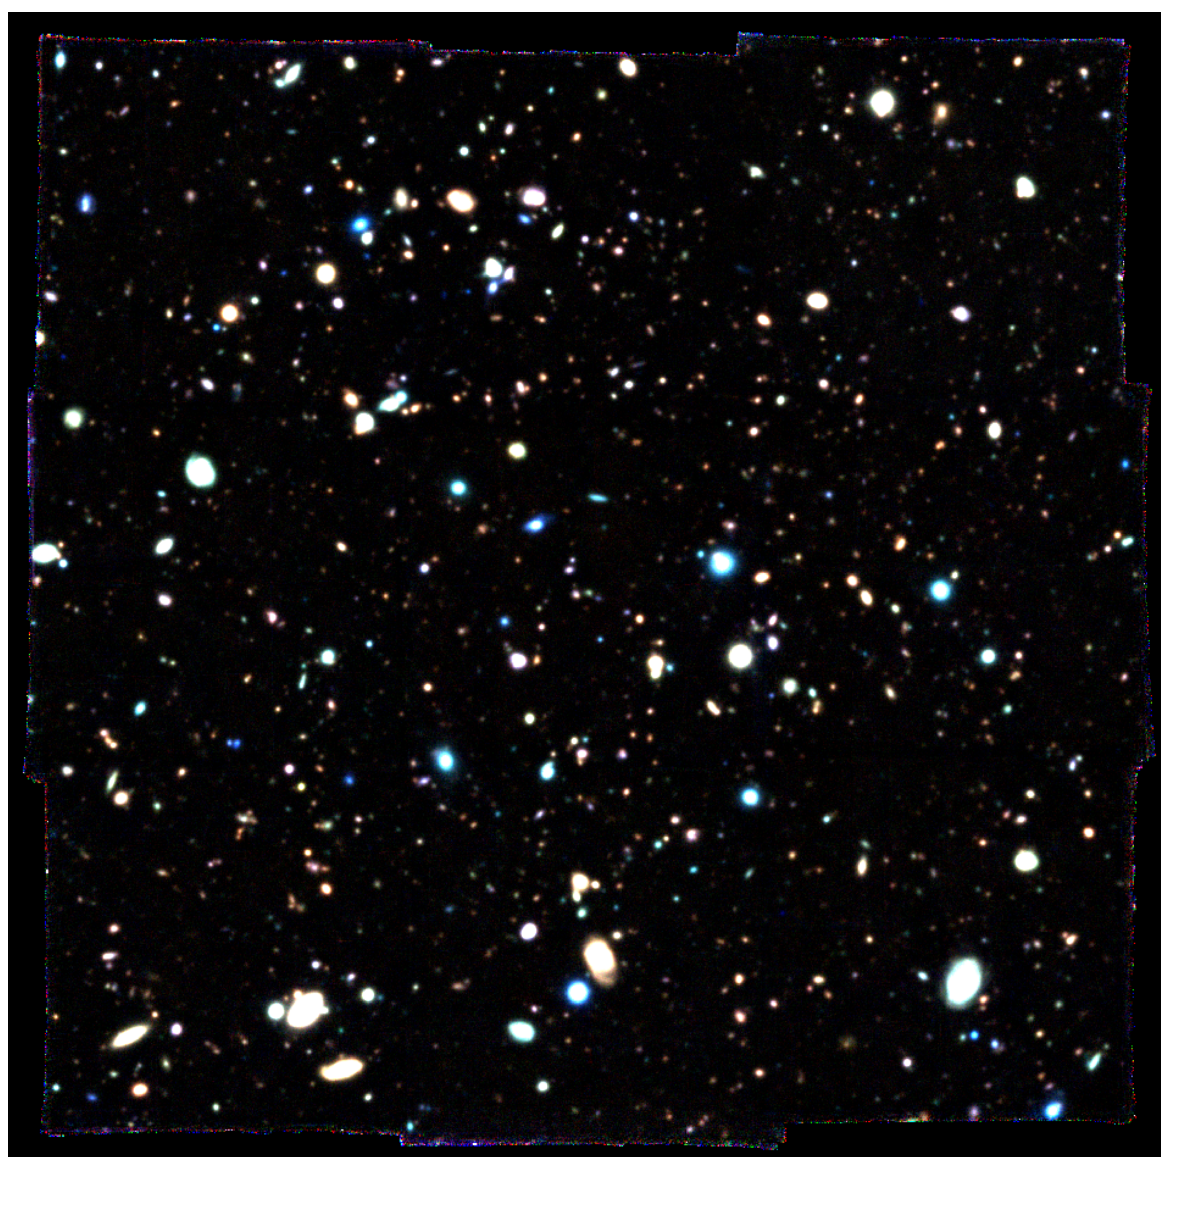
\includegraphics[width=\textwidth]{introduction/muse_colour_image}
    \captionsetup{justification=justified}    
    \caption{MUSE HUDF}               
    \label{fig:muse_colour_image}
  \end{subfigure}
  %
  \begin{subfigure}[b]{0.4\textwidth}
    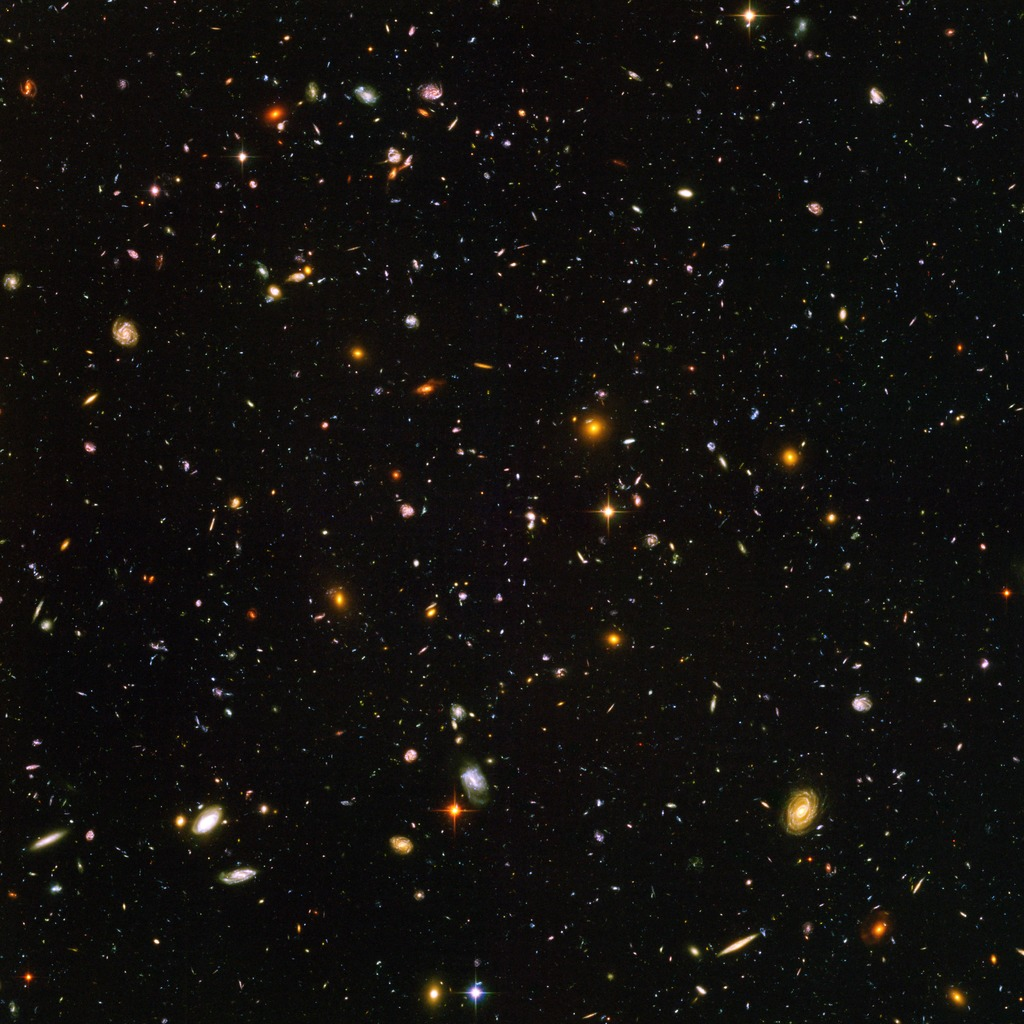
\includegraphics[width=\textwidth]{introduction/hubble_ultra_deep_field}
    \captionsetup{justification=justified}    
    \caption{HST HUDF}
    \label{fig:hubble_ultra_deep_field}
  \end{subfigure}
  \captionsetup{justification=justified}
  \caption[Hubble Ultra Deep Field]{(a) A colour image created from the MUSE spectroscopic data of the HUDF. The wavelength range was split into three equal regions and then collapsed to create three bands (R, G, B). A final colour image was produced by combining these separate frames together. (b) The optical HUDF as captured by the Advanced Camera for Surveys instrument on the Hubble Space Telescope \cite{hudf_image}. }
  \label{fig:hst_muse_hdf}
\end{figure}

\twocolumngrid

asdasd

\subsection{Project Aims}
This paper discusses the study undertaken to understand the dynamics between the gas and stars in galaxies. Data extraction is performed on a MUSE data cube, the sample is reduced, and various fittings are then applied to the data set. 

In Section \ref{sec:analysis}, the methodology of the galaxy extraction from the MUSE cube is discussed, as well as the subsequent analysis performed by applying different fitting routines: O[II] Gaussian doublet fittings, Voigt profile fittings, and fitting with a penalised pixel-fitting method (pPXF). Following this, Section \ref{sec:discussion} provides an exploration on the implications on the results obtained from the data analysis. Then the discussion will end on future work which can be performed to extend on the project.

\section{Analysis} 
\label{sec:analysis}

The goal in the analysis was to reduce down individual galaxy spectra to then apply fitters which would provide a way to compare the stars in a galaxy to the gas within it. 

\subsection{Cube extraction}

To begin with, galaxies were extracted from the 3D MUSE data cube so that they could later be manipulated. This process involved  

\onecolumngrid

\begin{figure}
  \begin{subfigure}[b]{0.495\textwidth}
    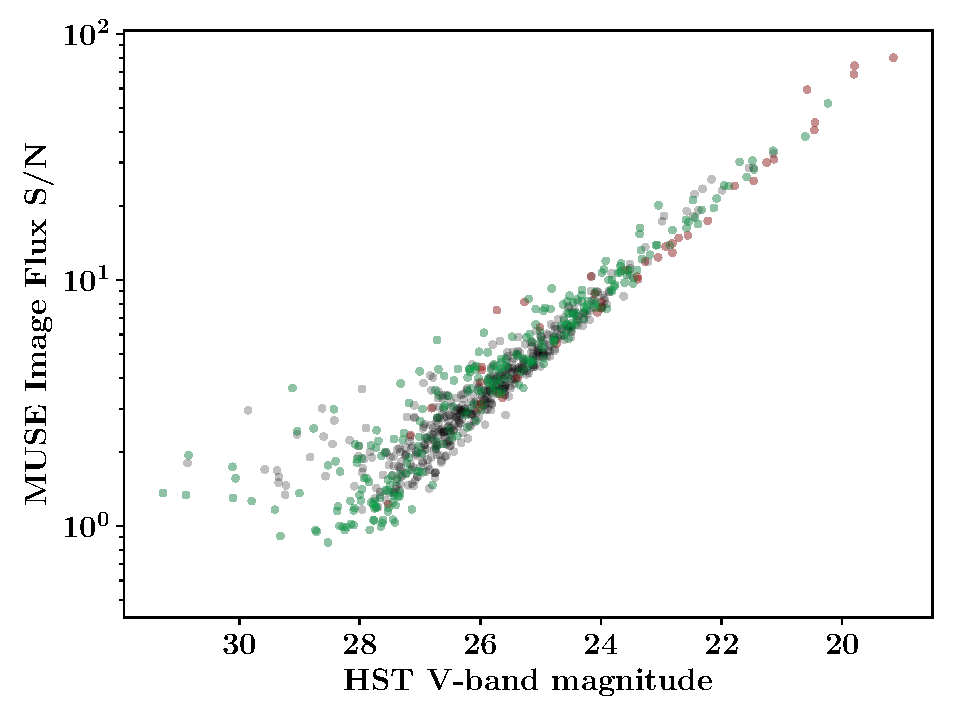
\includegraphics[width=\textwidth]{data/image_sn_vs_vband}
    \captionsetup{justification=justified}
    \caption{Image S/N vs. V-band}
    \label{fig:image_sn_vband}
  \end{subfigure}
  %
  \begin{subfigure}[b]{0.495\textwidth}
    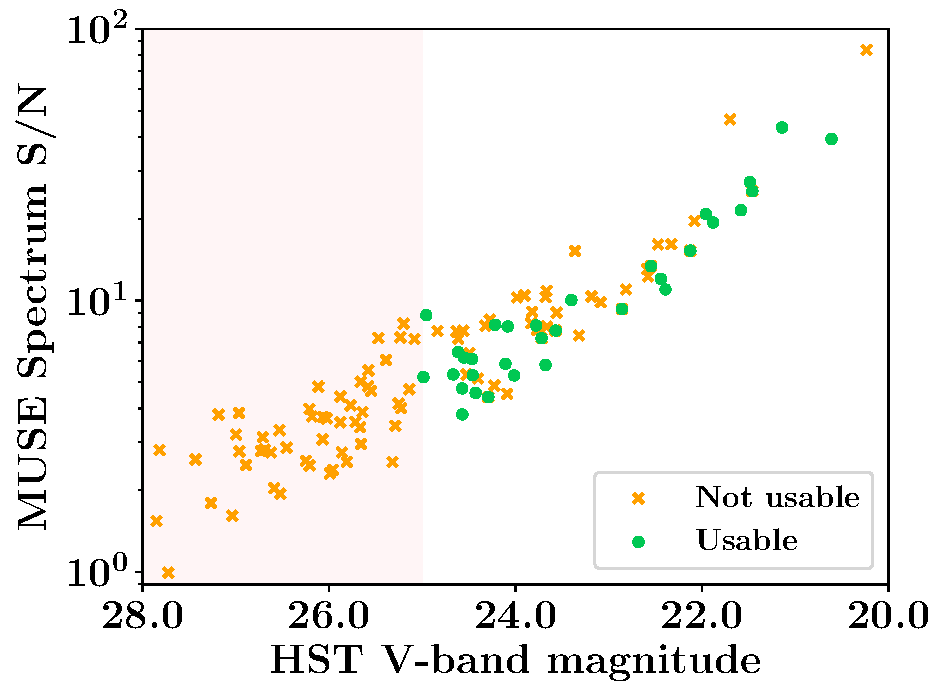
\includegraphics[width=\textwidth]{data/sn_vs_vband}
    \captionsetup{justification=justified}    
    \caption{Spectroscopic S/N vs. V-band}
    \label{fig:spec_sn_vband}
  \end{subfigure}
  \captionsetup{justification=justified}
  \caption[HUDF Objects]{(a) The signal-to-noise of the image flux for every object in the MUSE collapsed image plotted against their respective V-band magnitudes from the HST catalogue. The red points represent those with redshifts $z<0.3$, and the green points are a chosen sample of 300 points as defined by the sextractor probability that they are not stars. (b) }
\end{figure}

% FINISH OFF THE CAPTION FOR THE ABOVE

\twocolumngrid

asdasd

\begin{center}
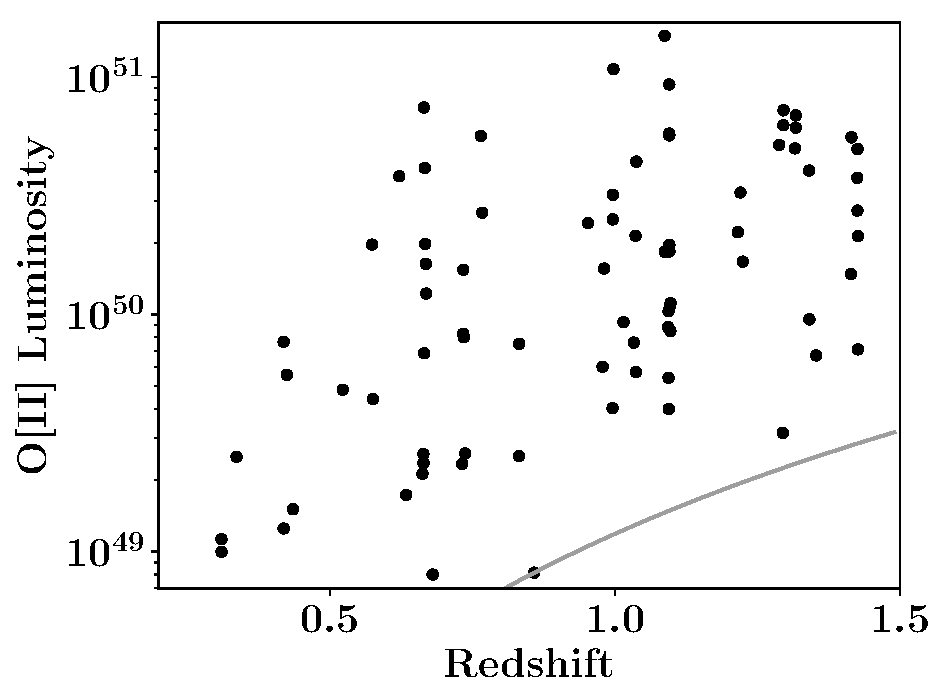
\includegraphics[width=1.0\linewidth]{data/o_ii_luminosity_vs_redshift}
\captionof{figure}[OII Luminosity vs. Redshift]{Graph showing the calculated luminosity for the O[II] doublet plotted against redshift. Data points are plotted as well as a model line representing the lower-limit of the flux from the sample. [???]a}
\label{fig:oiiluminosity_redshift}
\end{center}

aasdasd

\subsection{Line fittings and pPXF} 

After extracting the individual galactic objects from the main MUSE cube, the data had to be verified and then fitted using two different routines: (i) O[II] doublet fitting, and (ii) pPXF absorption line fitting. 

\subsubsection{Gaussian doublet fitting}

sdfasdfas

\subsubsection{Voigt fitting}

sadfasd

\begin{center}
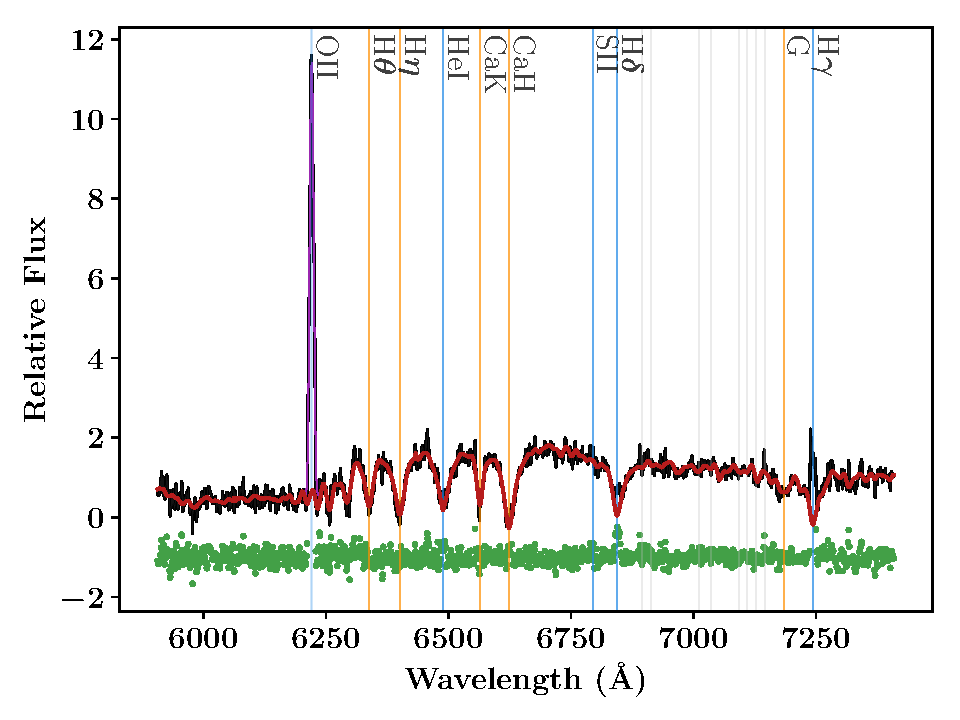
\includegraphics[width=1.0\linewidth]{data/cube_1804_fitted}
\captionof{figure}[OII Luminosity vs. Redshift]{Fitting of a galaxy spectrum with pPXF.}
\label{fig:oiiluminosity_redshift}
\end{center}

\begin{center}
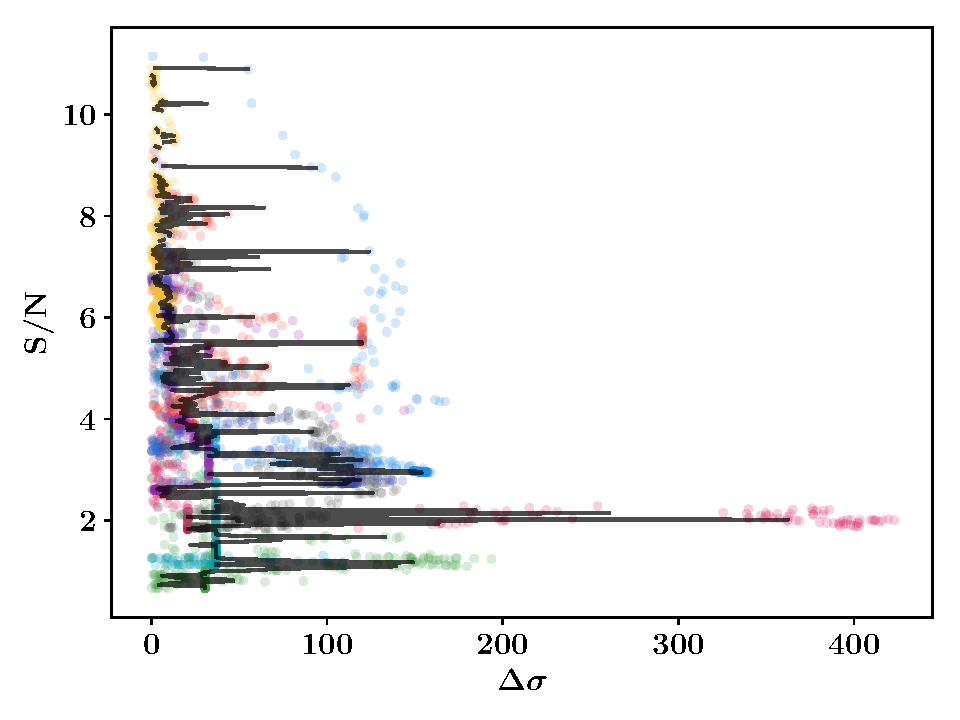
\includegraphics[width=1.0\linewidth]{data/reprocessed_sn_vs_delta_sigma}
\captionof{figure}[S/N vs. delta(sigma)]{The signal-to-noise versus the fractional error of the $\sigma$ line width of the pPXF curve fittings.}
\label{fig:oiiluminosity_redshift}
\end{center}

\section{Discussion} 
\label{sec:discussion}

sadfsadfsadf

sdfasdfsdf

\section{Conclusions}
 
In conclusion, through extensive data and statistical analysis it can be said that the dynamics of stars and gas in galaxies are ... (?) 

\begin{acknowledgments}
The author would like to thank Dr.~M.~Swinbank and Alfie Tiley for their continual help and support throughout the project period, without which, the project would have been experimentally grounded.
\end{acknowledgments}

\bibliographystyle{unsrt}
\bibliography{stars_gas_dynamics}

\end{document}